In this section we hypothesize and test a condition for shock formation.
This condition is empirically motivated, but leads to quantitatively accurate
predictions and can be motivated by simple arguments.

We will make use of the arithmetic and harmonic averaging operators, 
denoted by a bar and a hat, respectively:
\begin{align*}
\bar{f} & = \int_0^1 f(x) dx & \hat{f} & = \left(\int_0^1 \frac{1}{f(x)} dx\right)^{-1}.
\end{align*}

\subsection{Effective wave speeds}
In a homogeneous medium, small-amplitude perturbations travel at the
characteristic speed
\begin{align*}
c(\sigma_0) = \sqrt{\frac{\sigma'_0(\epsilon)}{\rho}} \ \ \ 
\mbox{ where } \sigma'_0(\epsilon)=\left.\sigma'(\epsilon)\right|_{\sigma=\sigma_0},
\end{align*}
where $\sigma_0$ is the stress in the ambient state.
In particular, in the linear case
these velocities are equal to the sound speed:
\begin{align} \label{hom_sound_speed} 
\sigma(\epsilon) & = K \epsilon  \implies
c =  \sqrt{K/\rho}. \end{align}

%Although we are interested in nonlinear propagation, it is helpful to
%review first some aspects of linear wave propagation, taking
%$\sigma(\epsilon,x)=K(x)\epsilon$.
%In a homogeneous medium, linear waves travel at the characteristic velocity
%(sound speed)

Now let us consider a linear periodic medium.  A pulse in such a medium
will spread out over time due to reflections.
The fastest moving part is that which is unreflected; this part travels at
the harmonic average of the sound speed:
\begin{align} \label{cmax}
\hat{c} = \left(\int_0^1{\sqrt{\frac{\rho(x)}{K(x)}} dx}\right)^{-1}.
\end{align}
Meanwhile, the main part of the signal (for a long-wavelength pulse) travels
at the effective sound speed given by using the average of the density and the
harmonic average of the bulk modulus \cite{santosa1991}:
%{\bf won't a discontinuity also travel at this speed? So
%nothing to do with wavelength?}
\begin{align} \label{ceff}
c_\textup{eff} = \sqrt{\frac{\Kmean}{\rhomean}}
\end{align}
%where we use an overbar to indicate the mean and a hat to indicate the
%harmonic mean:
%\begin{align}
%\rhomean & = \frac{1}{2}(\rho_A + \rho_B) &
%\Kmean & = 2 \left(\frac{1}{K_A} + \frac{1}{K_B}\right)^{-1}.
%\end{align}
The effective velocity \eqref{ceff} is smaller than the maximum bulk
velocity \eqref{cmax},
due to the macroscopic slowing effect of repeated reflections.
%Given an initial small pulse, at later times most of the energy in the
%pulse will be found at a location determined by $c_\textup{eff}$.
%However, smaller portions of the pulse will have spread out; the fastest-traveling
%portion is that which undergoes no reflections and moves at speed $\hat{c}$.
%given by the harmonic average of the homogeneous material sound speeds:
%\begin{align} \label{cmax}
%\cmean = 2\left(\frac{1}{c_A} + \frac{1}{c_B}\right)^{-1}.
%\end{align}

By similar reasoning, small-amplitude perturbations traveling
in a nonlinear periodic medium with ambient stress $\sigma_0$
can be shown to travel at an effective velocity
\begin{align*}
c_\textup{eff}(\sigma_0) & = \pm\sqrt{\frac{\widehat{\sigma'_0}}{\rhomean}}
& \mbox{where }
\sigma'_0 & = \left. \frac{\partial \sigma(\epsilon,x)}{\partial \epsilon}\right|_{\sigma=\sigma_0}.
\end{align*}
%\begin{align}
%\widehat{\sigma'_{0}}=\left(\int_0^1 \left(\left.\frac{\partial \sigma(\epsilon,x)}{\partial \epsilon}\right|_{\sigma=\sigma_0}\right)^{-1} dx \right)^{-1}
%\end{align}

%\begin{align}
%\left<\sigma'\right> & = 2 \left(\frac{1}{\sigma'_{0,A}} + \frac{1}{\sigma'_{0,B}}\right)^{-1}
%\end{align}
%and
%\begin{align}
%\sigma'_{0,A}=\left.\sigma'(\epsilon)\right|_{\sigma=\sigma_0}
%\end{align}

Now consider the case of a shock separating two constant states $q_l,q_r$
in the nonlinear medium, and let $[q]$ denote the jump $q_r-q_l$.  Since it will experience reflections at the 
material interfaces, the shock may conceivably break up into many smaller
discontinuities, as it clearly would in the linear case.  If the shock
is able to persist as a single large discontinuity (due to nonlinear
compression), we might expect that it will also travel at an effective 
velocity; it is natural
to suppose that this velocity will be related to the Rankine-Hugoniot shock
speed in the same way that the effective velocities above are related to
the characteristic speeds.  The R-H jump conditions in a homogeneous medium
give the shock speed
\begin{align} \label{shockspeed}
s = \sqrt{\frac{[\sigma]}{[\epsilon]\rho}}.
\end{align}
Thus it is natural (based on \eqref{ceff}) to consider an "effective shock speed"
\begin{align} \label{effshockspeed}
s_\textup{eff} = \sqrt{\widehat{\left(\frac{[\sigma]}{[\epsilon]}\right)}\frac{1}{\rhomean}},
%s_\textup{eff}(\sigma_l) = \pm\sqrt{\left<\left(\frac{[\sigma]}{[\epsilon]}\right)^{-1}\right>\frac{1}{\rhomean}}
\end{align}
%where
%\begin{align}
%\left<\sigma_l/\epsilon_l\right> & = 2 \left(\frac{\epsilon_{l,A}}{\sigma_{l,A}} + \frac{\epsilon_{l,B}}{\sigma_{l,B}}\right)^{-1}
%\end{align}
which we propose as an estimation of the velocity at which the 
largest portion of the jump may travel.  Smaller parts of the shock will 
have spread out due to being reflected more or fewer times.  The fastest-travelling
portion is that which undergoes no reflections.
%This portion will travel at a velocity given by the harmonic average $\hat{s}$ 
%of the shock speed defined in \eqref{shockspeed}.  
The strength of this "purely transmitted" 
shock diminishes exponentially in time, so that to a good approximation it travels
at the speed for non-reflected small perturbations in the state ahead of the shock:
$$\hat{c}(\sigma_r) = \left(\int_0^1 \left(\frac{\sigma'_r(x)}{\rho(x)}\right)^{-1/2}dx\right)^{-1}.$$

%Consider propagation of a shock in some characteristic family in the periodic
%medium.  Part of the shock will move ahead at  the harmonic average of the ambient
%sound speed:
%$$\hat{c}(\sigma_0) = \left(\int_0^1 \left(\frac{\sigma'_0(x)}{\rho(x)}\right)^{-1/2}dx\right)^{-1}.$$
\subsection{A generalized entropy condition}
A generalized condition for shock stability can be motivated as follows.
The bulk of the shock will advance at speed $s_\textup{eff}$.  If 
$s_\textup{eff}<\hat{c}(\sigma_r)$ then the bulk of the shock will fall behind
the leading (weak) bit.  This will make the main shock weaker, causing it to 
propagate even more slowly, so that more of the strength of the shock will
"escape" ahead of it.  Hence the shock will be converted
into many weak shocks after some time.  
%{\bf One way to make this more
%rigorous would be to quantify the rate of decay of the shock in some sense.}

This proposed condition for shock persistence in the periodic medium can be 
viewed as a generalization of the Lax entropy condition for shocks.  Namely, 
characteristics of the corresponding family must impinge on the shock.
In our case, the characteristic speed involved in this condition is the
harmonic average of the sound speed ahead of the shock.
The relevant shock speed is the effective shock speed $s_\textup{eff}$ 
from \eqref{effshockspeed}.

The effective shock speed for various values of $Z_B$ (with $\rho_B=K_B=Z_B$)
and a range of stresses 
$\sigma_l$ is plotted in Figure \ref{fig:cshock}.  Here we have taken
$\sigma_r=0$, so that $\hat{c}(\sigma_r)=1$.  Hence we expect shock stability
for a given impedance $Z_B$ and left state $\sigma_l$, if the corresponding 
effective shock speed \eqref{effshockspeed}
is greater than unity.
For the homogeneous medium ($\rho_B=K_B=Z_B=1$),
the effective shock speed is just the ordinary shock speed, and any shock 
is of course predicted to be stable.  However, for heterogeneous media, 
small-amplitude shocks have effective velocity less than one, 
so that effective characteristics do not impinge on the shock from the right.

\begin{figure}
\centerline{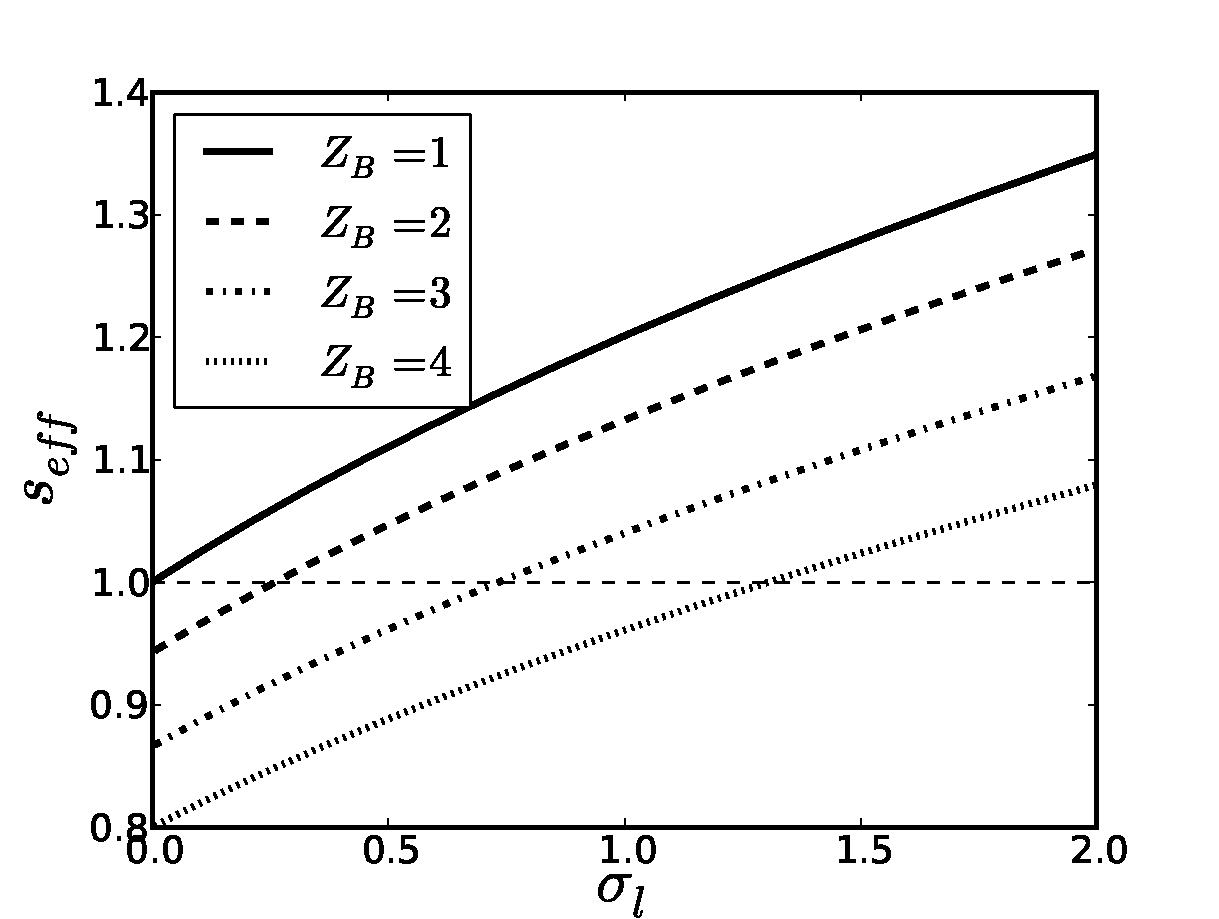
\includegraphics[width=4in]{figures/seff.pdf}}
\caption{Effective shock speed \eqref{effshockspeed} as a function of stress behind the shock.\label{fig:cshock}}
\end{figure}

Based on the foregoing theory, we can define a critical parameter that
we will refer to as the {\em relative effective shock speed}:
\begin{align} \label{eq:seff}
S_\textup{eff} & = \frac{s_\textup{eff}}{\hat{c}(\sigma_r)}.
\end{align}
Notice that $S_\textup{eff}$ depends on the ambient states $\sigma_r,\sigma_l$
as well as the material parameters $\rho(x),\sigma'_r(x)$.  We expect that a
shock will form whenever $S_\textup{eff}$ exceeds unity.

\subsection{Numerical validation}
The true dynamics of a propagating front in the periodic medium
is generally much more complicated than what we have just considered,
since such a front quickly results in many reflected/transmitted shocks and
rarefactions in mutual interaction.  Nevertheless, simulations of
low-contrast media and large-amplitude initial conditions do lead to
persistent large-amplitude shock fronts, whereas simulations of 
higher-contrast media or smaller-amplitude initial conditions such
shocks are not visibly apparent.  For the former case, we have compared directly 
the apparent shock velocity with the predicted value $s_\textup{eff}$.
There is some ambiguity in determining the precise location of the shock,
since the front structure is complex, but in general agreement to within
1-3\% is observed for the range of materials and initial conditions considered
in this work.
%This is a very rough qualitative
%confirmation of the general implications of the theory.

We now conduct two tests to quantitatively validate this theory.
In the first, we test whether shocks form from smooth initial conditions.
The initial condition consists of
two uniform initial states separated by a thin smooth transition region:
\begin{align*}
u(x,0) & = 0, \\
\sigma(x,0) & = \begin{cases} \sigma_l & x \le 30 \\
                        \sigma_l \exp(-(x-30)^2) & x>30.
                \end{cases}
\end{align*}
%This theory is tested as follows.  The initial condition consists of a 
%large region where $\sigma=2\sigma_l$, a region with $\sigma=0$, and
%between them a rapid (but smooth) transition region.  The stressed region
%resolves itself into left- and right-going pulses, each of which has
%$\sigma=\sigma_l$.  
The solution is evolved to time $t=100$, well beyond
the time for shock formation in a homogeneous medium for all of the initial
states studied.  Then the velocity
is reversed and the simulation continues to $t=200$.  The final entropy 
and initial entropy are compared to determine whether shock formation has
occurred.  In Figure \ref{fig:ent_cshock}, the ratio of final and initial 
entropies is plotted for many tests over the ranges 
$1.5\le\rho_B\le 9,1\le K_B \le 4,0.1\le\sigma_l\le4$, 
and $\sigma_r=0$.  The results are in very good agreement with the theory;
i.e. entropy loss occurs when $S_\textup{eff}>1$
and generally is on the level of numerical error otherwise.  
%Some small entropy loss is observed when the impedance contrast is large
%and $1-S_\textup{eff}$ is very small, suggesting that the foregoing
%approximate theory may be less accurate for large impedance ratios.

\begin{figure}
\centerline{
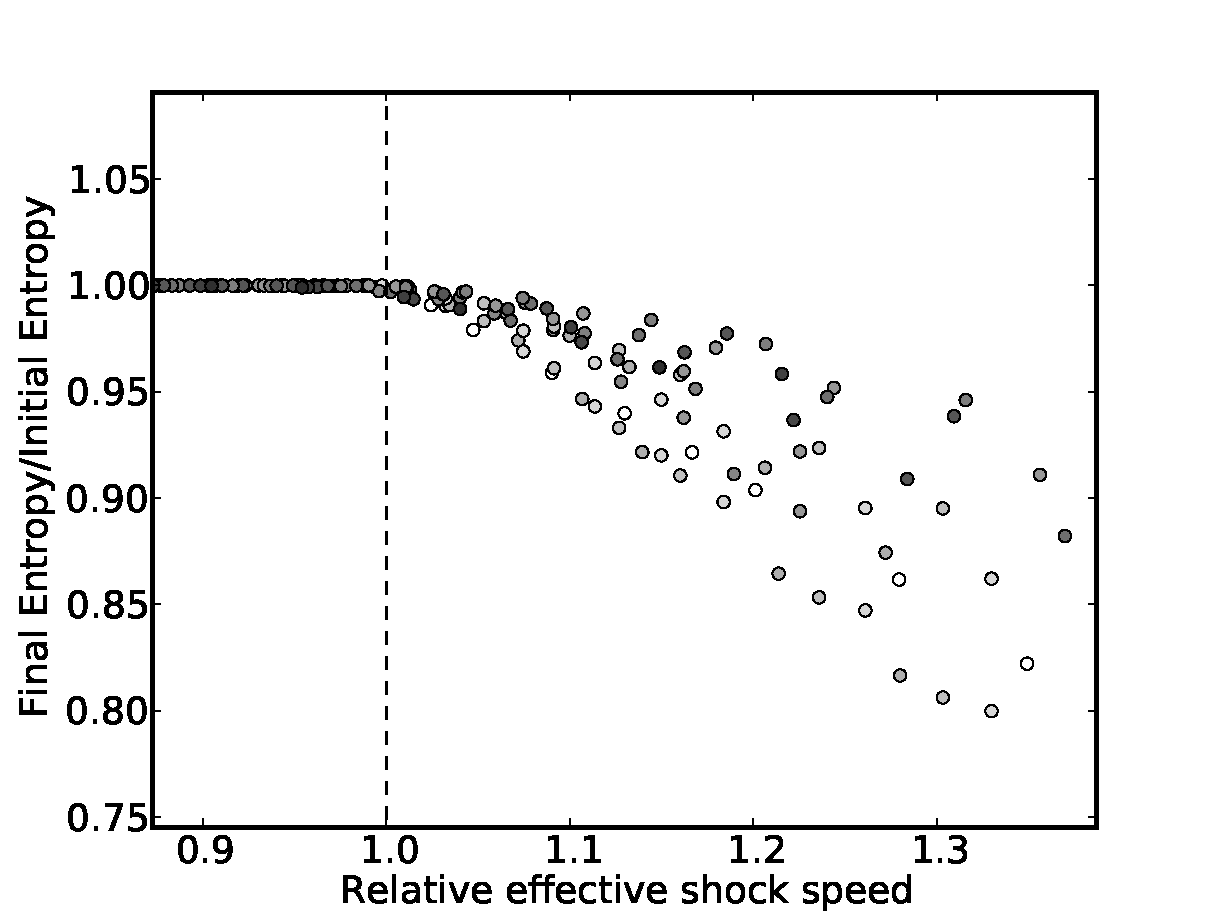
\includegraphics[width=4in]{figures/ent_cshock.pdf}}
\caption{Relative entropy versus relative effective shock speed $S_\textup{eff}$
\eqref{eq:seff} 
for a wide range of materials and initial conditions.  Notice that the 
entropy is near constant for $S_\textup{eff}<1$ (indicating
no shock formation), and decreasing for $S_\textup{eff}>1$ (indicating
shock formation).  The shade of each point indicates the impedance contrast
on a logarithmic scale, with darker points corresponding to higher impedance
contrast.
\label{fig:ent_cshock}}
\end{figure}


%{\bf The theory still needs to be checked for cases with $\sigma_r\ne 0$.
%Also, I want to somehow emphasize that Figure 12 is a projection of a 4-dimensional
%space.
%%Additionally, need to check if this theory still proves correct for
%%very large $Z$ and $\sigma_l$.  This requires modification of the
%%initial condition to prevent rapid shock formation within a single
%%layer.
%Also, I want to do a longer-time and higher-resolution test to make the behavior
%clearer.}

In the second test, we start with discontinuous initial conditions and
study the entropy evolution in time.  There is some difficulty in choosing
an initial condition.  Using a pure right-going shock in one material quickly 
leads to very strong reflections.  Instead,
we use an initial condition consisting of an "effective shock", where the
left and right states are related by the usual Rankine-Hugoniot conditions
but with the material parameters $\rho,K$ replaced by the effective parameters
$\rhomean,\Kmean$.  Specifically, we take $(\sigma(x,0),u(x,0))=0$ for $x>30$
and $(\sigma(x,0),u(x,0))=(\sigma_l,u_l)$ for $x\le 30$, where
\begin{align*}
u_l & =-\sqrt{\frac{\sigma_l \log(\sigma_l+1)}{\rhomean\Kmean}}.
\end{align*}
This dramatically reduces the severity of initial reflections of the front,
which seems advantageous for our purpose of studying shock propagation.

The total entropy evolution versus time is plotted in Figure \ref{fig:ent_cshockic}
for a range of values of $\sigma_l$ and a medium with $Z_B=\rho_B=K_B=2$.  
The legend indicates the corresponding values
of the relative effective shock speed $S_\textup{eff}$.  In all cases there
is a rapid but small initial entropy loss.  However, for $S_\textup{eff}<1$
the entropy is nearly constant after this initial time.  On the other hand, for
$S_\textup{eff}>1$ the entropy continues to decrease significantly throughout the simulation.

\begin{figure}
\centerline{
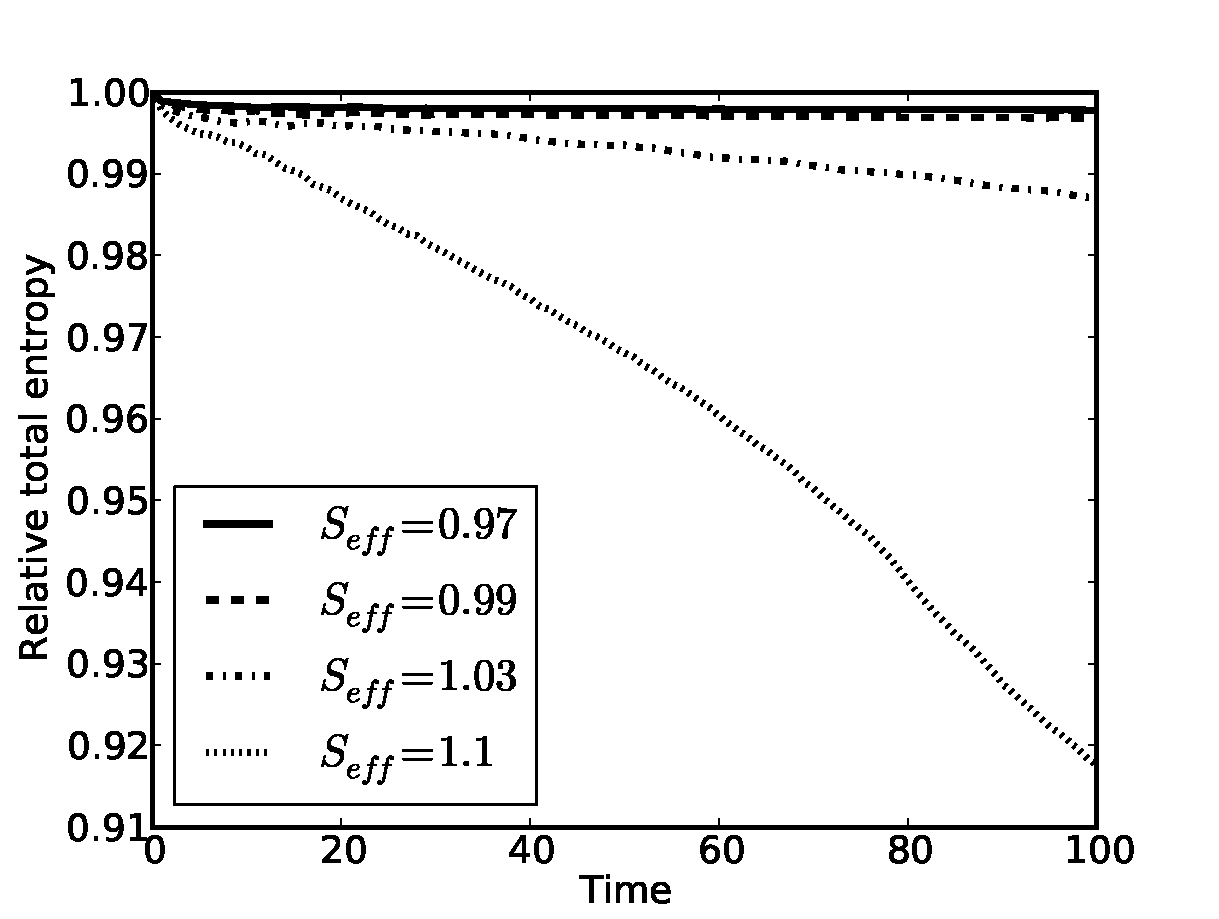
\includegraphics[width=4in]{figures/shock_ic_entropy_Z2.pdf}}
\caption{Entropy as a function of time (relative to initial entropy)
for a range of relative effective shock speeds $S_\textup{eff}$ \eqref{eq:seff}.
The medium has $\rho_B=K_B=Z_B=2$.
Notice that the entropy is nearly constant (after a brief initial decrease) for
$S_\textup{eff}<1$, and decreasing for $S_\textup{eff}>1$.\label{fig:ent_cshockic}}
\end{figure}

Figure \ref{fig:ent_cshockic2} shows similar results for a medium with
$Z_B=\rho_B=K_B=4$.  In this case, we see that for $S_\textup{eff}$ slightly
less than 1, some significant entropy loss continues after the initial
period.  The entropy loss is much more significant when $S_\textup{eff}>1$.
%Again we see that the theory proposed here seems to be accurate for
%smaller impedance contrasts, but less accurate as the impedance contrast
%is increased.


\begin{figure}
\centerline{
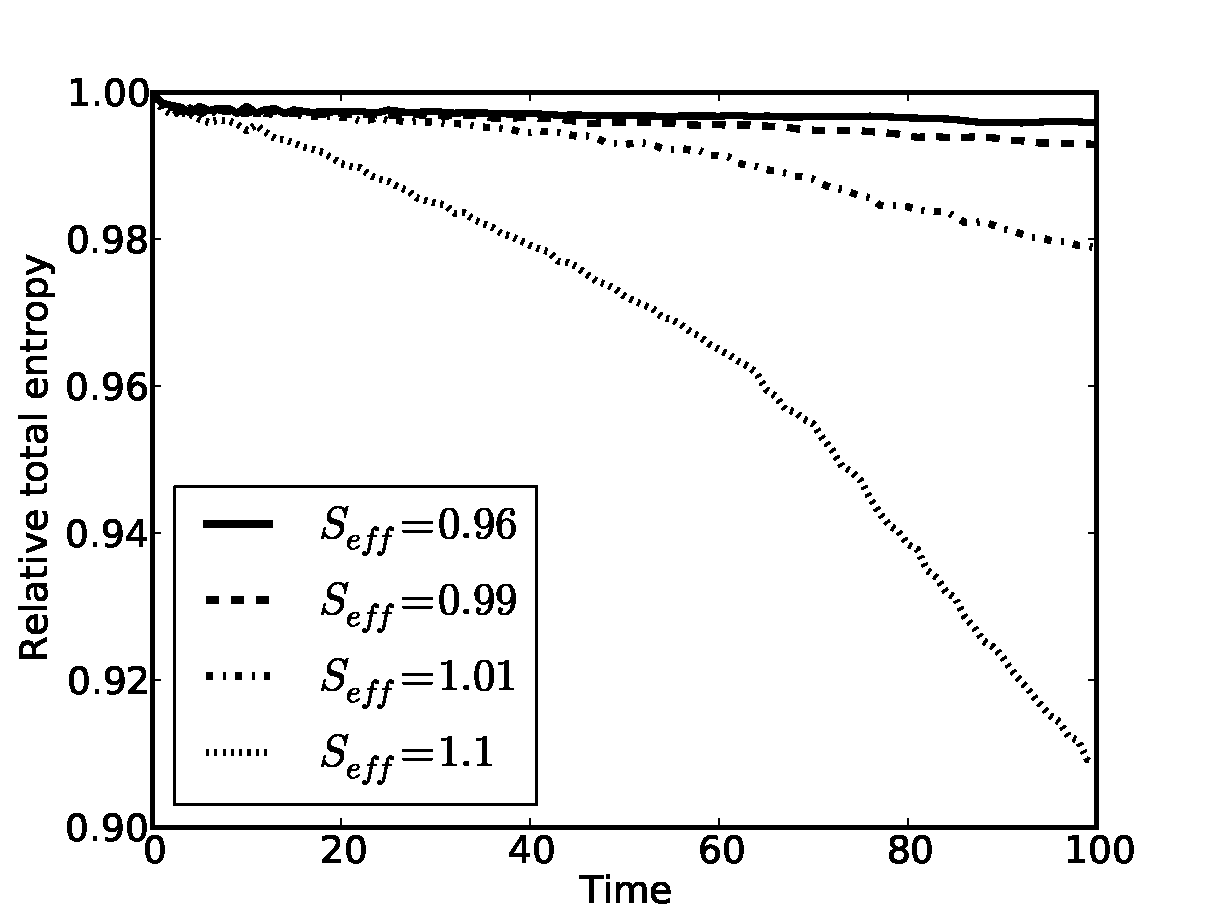
\includegraphics[width=4in]{figures/shock_ic_entropy_Z4.pdf}}
\caption{Entropy as a function of time (relative to initial entropy)
for a range of relative effective shock speeds $S_\textup{eff}$ \eqref{eq:seff}.
The medium has $\rho_B=K_B=Z_B=4$.
Notice that the entropy is nearly constant (after a brief initial decrease) for
$S_\textup{eff}<1$, and decreasing for $S_\textup{eff}>1$.\label{fig:ent_cshockic2}}
\end{figure}


